% DO NOT COMPILE THIS FILE DIRECTLY!
% This is included by the the driver file (FlipBeamerTemplate.tex).


{%% This is a total kludge for a fancy title page background
%\vspace{1.5em}
\setbeamertemplate{sidebar right}{\llap{
\includegraphics[width=\paperwidth,height=\paperheight]{Opening}}}
\begin{frame}[c]%{\phantom{title page}} 
% The \phantom{title page} is a kludge to get the red bar on top
% \titlepage
\begin{center}
	
	\vspace{10em}
	\footnotesize\textcolor{gray}{PhD Monitoring: 	\texttt{Felipe Maldonado}}
	\vspace{.5em}
	
	
	
\includegraphics[height=1.5cm]{logoANU2011}\\
	\textcolor{anugold}{\textit{Australian National University}, \today}

\end{center}
\end{frame}
}

{
\setbeamertemplate{sidebar right}{\llap{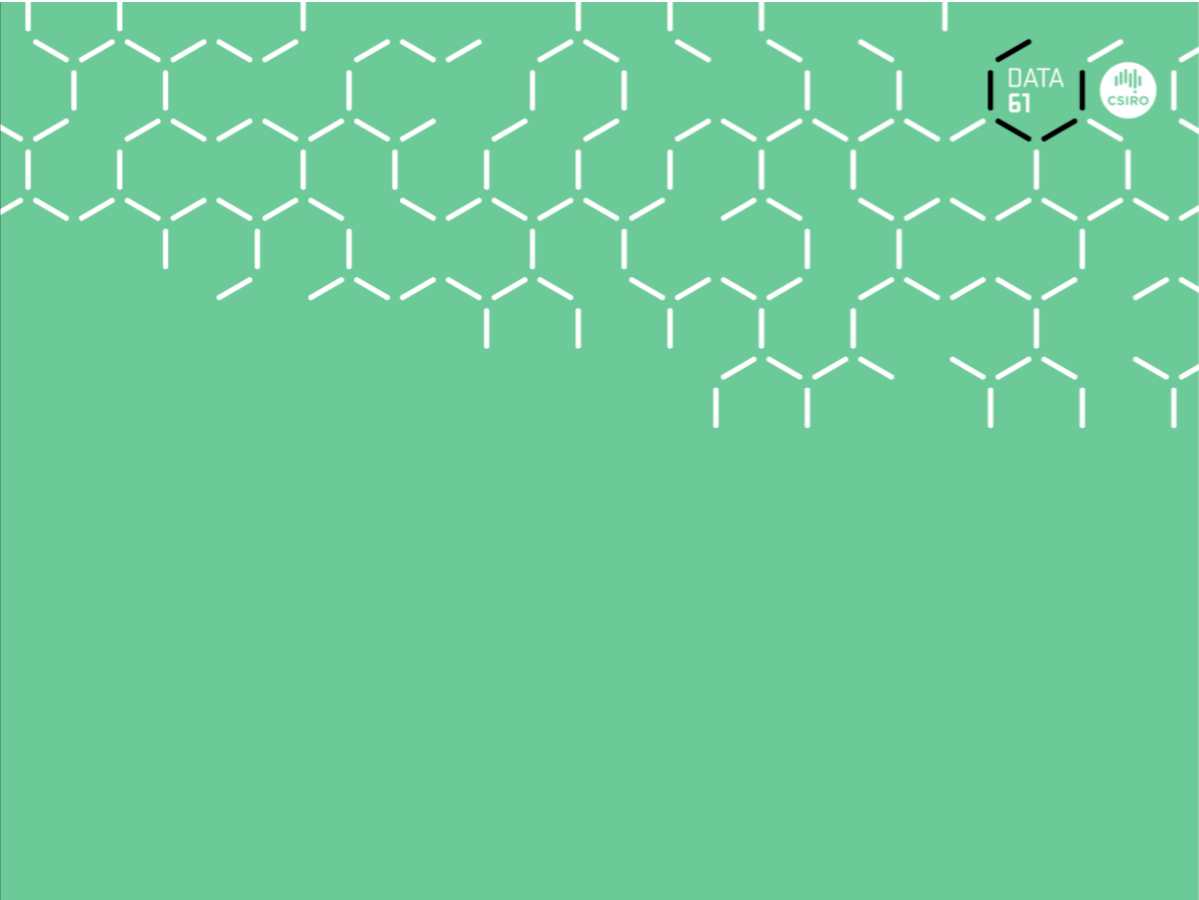
\includegraphics[width=\paperwidth,height=\paperheight]{separator}}}
\begin{frame}[c]


\vspace{7em}
\textcolor{anugold}{\textit{Panel:}}
\begin{itemize}
\item Pascal Van Hentenryck (Supervisor) 
\item Lexing Xie (Chair)
\item Patrik Haslum
\item Gerardo Berbeglia
\end{itemize}
\end{frame}
}

 %%%%% MOTIVATION %%%%%
\begin{frame}[c]{Motivation}{}
	Plenty of markets where social influence is relevant in the customer`s choices. 
	\begin{columns}[t]
	\begin{column}[T]{5.5cm}
		\begin{itemize}
			\item 1
			\item 2		
		\end{itemize}
	\end{column}
	
	\begin{column}[T]{5.5cm}
		\begin{itemize}
			\item 3
			\item 4		
		\end{itemize}
	\end{column}
	\end{columns}
	\begin{alertblock}{MusicLab Experiment. Salganik et al. (2006)}
		Inequality and unpredictability in a cultural market. Negative effects of social influence.
	\end{alertblock}
	\end{frame}
	
	
	%%%%%%%SEPARATION%%%%%
\addtocounter{framenumber}{-1}
{	
\setbeamertemplate{sidebar right}{\llap{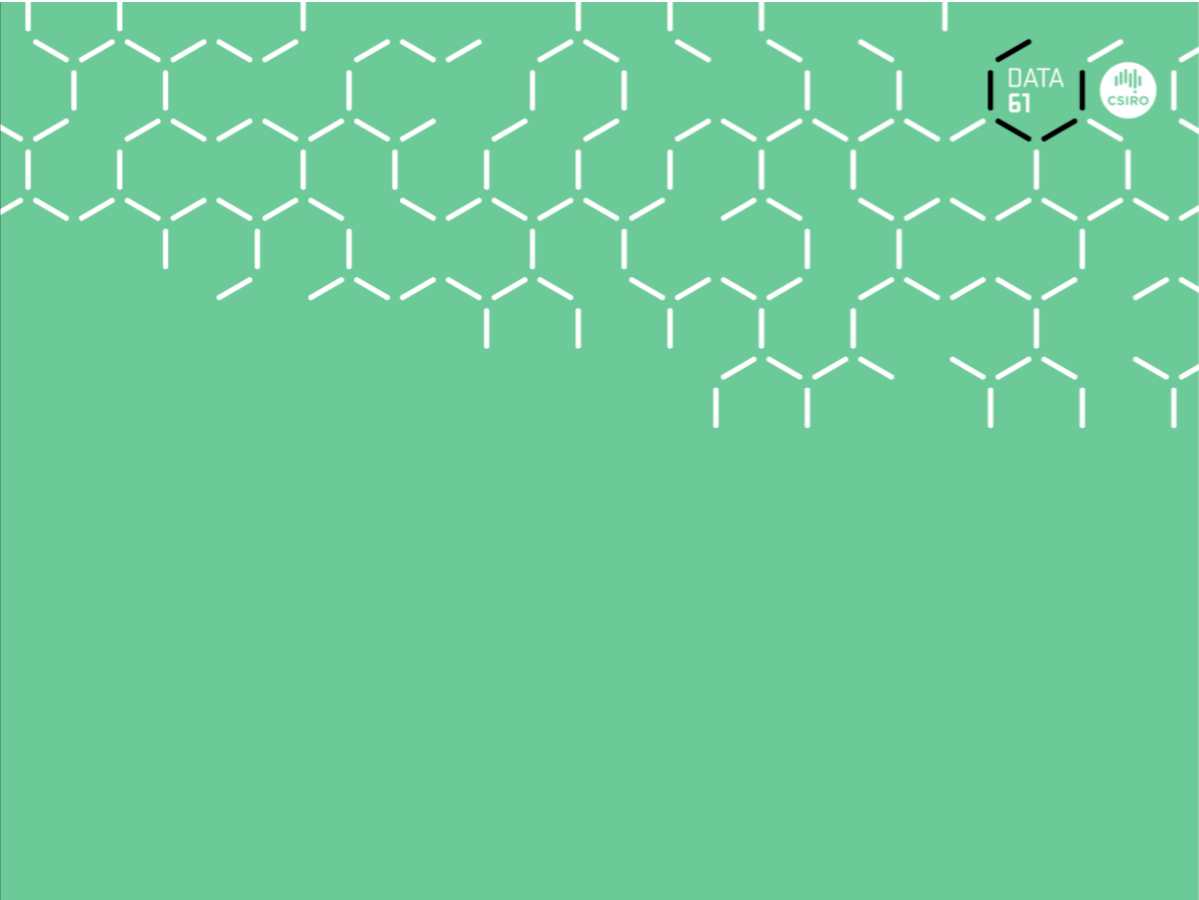
\includegraphics[width=\paperwidth,height=\paperheight]{separator}}}
\begin{frame}[c]
\begin{center}

	\vspace{10em}
	 
\includegraphics[height=1.5cm]{Model}\\
	\vspace{.5em}
	
\end{center}
\end{frame}
}
	
	

%%%%%%%MODEL AND ASSUMPTIONS 1 %%%%%%
\begin{frame}[c]{Model and assumptions}{}
	\begin{block}{Marketplace}
		A marketplace consists of a set $N$ of $n$ items. Each item $i\in N$ is characterized by two values:
		\begin{enumerate}
			\item its {\em appeal} $a_i > 0$,% which represents the inherent preference of trying item $i$;
			\item its {\em quality} $q_i > 0$.% which represents the conditional probability of purchasing item $i$ given that it was tried.
		\end{enumerate}	
	\end{block}

	\begin{alertblock}{Recovering qualities}
		Bernoulli sampling: $\hat{q}_{i,t}=\frac{d_{i,t}}{s_{i,t}}$
	\end{alertblock}
	
	\begin{block}{Rankings}
		 Each position $j$ of the ranking has a visibility $v_j$ which represents
the inherent probability of trying an item in position $j$.
	\end{block}
\end{frame}


%%%%%%%MODEL AND ASSUMPTIONS 2 %%%%%%

\begin{frame}[c]{Market share and social signals}

\begin{block}{Definition}
The market share of the product $i$ at stage $t\geq 0$ is given by:
$$\phi_{i,t}=\dfrac{d_{i,t}}{\sum_j d_{j,t}}, \mbox{if } t>0;\quad \phi_{i,0}=\dfrac{a_{i}}{\sum_j a_{j}} $$
\end{block}

Its evolution over time will depend (among others) of some social signal:
\end{frame}


%%%%%%%MODEL AND ASSUMPTIONS 3 %%%%%%
\begin{frame}[c]{Assumptions}

%\uncover<2->
%{ \alert{Proof:}
%The probability that item $i$ is purchased in the first step is given by
%\begin{equation*}
%p_i^{1st}(\phi) = \frac{v_i f(\phi_i)}{\sum\limits_{j=1}^n v_j f(\phi_j)} q_i.
%\end{equation*}
%The probability that item $i$ is purchased in the second step and
%no item was purchased in the first step is given by
%\begin{equation*}
%p_i^{2nd}(\phi) =\left( \frac{\sum\limits_{j=1}^n v_j f(\phi_j)(1-q_j)}{\sum\limits_{j=1}^n v_j f(\phi_j)} \right)\frac{v_i f(\phi_i)}{\sum\limits_{j=1}^n v_j f(\phi_j)} q_i.
%\end{equation*} 
%
%}

The probability that the customer
tries item $i$ is given by $P_i(\phi^t)$ where
\begin{equation}
\label{probatry}
P_i(\phi) =  \frac{v_{i} f(\phi_i)}{\sum_{j=1}^n v_{j} f(\phi_j)}
\end{equation}
and $f$ is a continuous, positive, and nondecreasing function. And $q_i$ is the conditional probability of downloading song if it was tried.

\begin{exampleblock}{Lemma 1}
The probability $p_i(\phi)$ that the next purchase is the product $i$
given the market share vector $\phi$ is given by
\begin{equation}
p_i(\phi) \ = \frac{ \overline{q}_i f(\phi_i)}{\sum_{j=1}^n \overline{q}_j f(\phi_j)} \label{probanext},
\end{equation}
where $\overline{q}_i=v_iq_i$
\end{exampleblock}

\end{frame}


%%%%%%%%SEPARATOR%%%%%%%%% BACKGROUND
\addtocounter{framenumber}{-1}
{	
\setbeamertemplate{sidebar right}{\llap{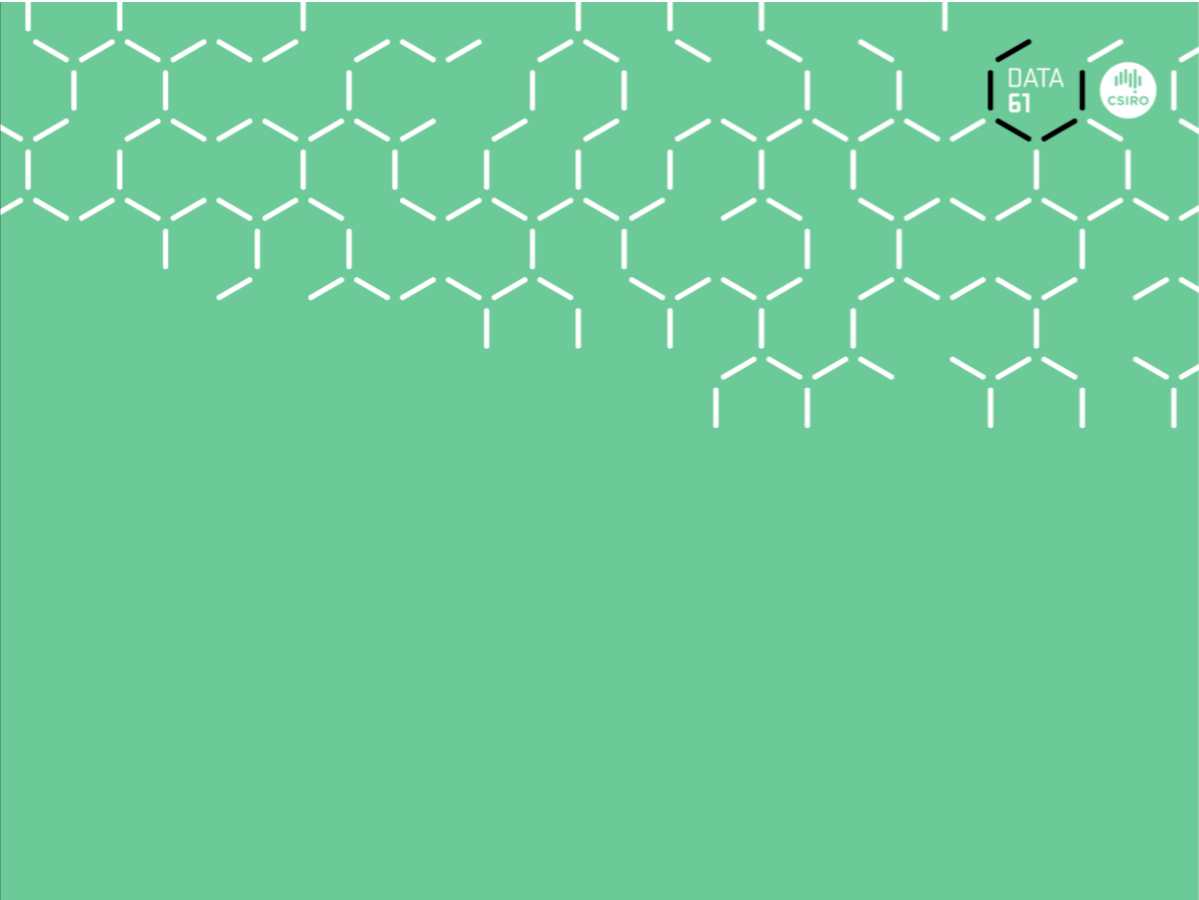
\includegraphics[width=\paperwidth,height=\paperheight]{separator}}}
\begin{frame}[c]
\begin{center}

	\vspace{10em}
	 
\includegraphics[height=1.5cm]{Background}\\
	\vspace{.5em}
	
\end{center}
\end{frame}
}
	
%%%%%% Stochastic Approx.	
 
\begin{frame}[c]{Stochastic approximation algorithms}
\begin{block}{Definition: Robbins-Monro Algorithm}A {\it Robbins-Monro
    Algorithm} (RMA) is a discrete time stochastic processes
  $\{x_k\}_{k \geq 0}$ whose general structure is specified by
\begin{equation}
\label{RMA}
x_{k+1}-x_k=\gamma_{k+1}[F(x_k)+U_{k+1}],
\end{equation}
\noindent	
where
\begin{itemize}
\item $x_k$ takes its values in some Euclidean space (e.g., $\R^n$ );
\item $\gamma_k$ is deterministic and satisfies $\gamma_k>0$,
  $\sum_{k \geq 1}\gamma_k=\infty$, and $\lim_{k \to\infty}\gamma_k=0$;
\item $F:\R^n\to\R^n$ is a deterministic continuous vector field;
\item $\EE[U_{k+1}| \Fk]=0$, where $\Fk$ is the natural filtration of
  the entire process.%\footnote{Because of this last condition on
%    $U^k$, a Robbins-Monro Algorithm is also known as a {\it
%      Martingale Difference Stochastic Approximation}.}
\end{itemize}
\end{block}
	
\end{frame}	
	
	
	
%%%%%%%% THE ODE METHOD



\begin{frame}[c]{The ODE Method}
Under certain conditions on $x_k$, $\gamma_k$, and $U_{k}$, the asymptotic
behavior of $x_k$ in Equation \eqref{RMA}, is closely related to the asymptotic behavior of the following continuous dynamic
process:
\begin{equation}
\label{RMC}
\frac{dx_t}{dt}=F(x_t), \quad x_t\in\R^n. 
\end{equation}

\begin{block}{Definition: Internally Chain Transitivity (ICT)}
A closed set $A$ is an ICT if for every $\epsilon>0$  and every $x,y\in A$ , there is a set $\{x_i\}_{i=0}^n\subset A$ such that $x_0=x, x_n=y$, and  $\|F(x_i)-x_{i+1}\|<\epsilon$, $\forall i\in\{0,...,n-1\}$.
\end{block}

\begin{exampleblock}{Theorem 1.}
Let $\{x_n\}_{n \geq 0}$ be a RMA \eqref{RMA}, where $F$ is of class $\mathcal{C}^2.$ %and some regularity conditions over $\gamma_t$ and $U_t$. 
Then,  with probability 1, the limit set $L\{x_n\}_{n \geq 0}$ is
  internally chain transitive for Equation \eqref{RMC}.
\end{exampleblock}

\end{frame}


%%%%%%%%%% DIFF EQUATIONS  DYNAMICAL SYSTEMS %%%%%


\begin{frame}[c]{Differential equations and dynamical systems.}
An {\it Initial Value Problem} (IVP) is given by a first-order autonomous system of
differential equations and a (vectorial) initial condition:
\begin{equation}
\label{cauchy}
\frac{dy}{dt}= F(y),\quad y(0)=x.
\end{equation}



\begin{block}{Definition: Equilibria}
A vector $y^*\in\mathbb{R}^n$ is an equilibrium for differential equation \eqref{cauchy} if $F(y^*)=0$.
\end{block}


\begin{block}{Definition: Stability}
  An equilibrium $y^*$ is said to be {\it stable} for Equation
  \eqref{cauchy} if, given $\epsilon > 0$, there exists $\delta > 0$
  such that $\| y(t) - y^* \| < \epsilon$ for all $t > 0$ and for
  all $y$ such that $\|y - y^*\| < \delta$.
  We say that $y^*$ is {\it asymptotic stable} if  also satisfies \[
\lim_{t\to\infty}y(t)=y^*.
\] 
\end{block}

\end{frame}

%%%%% EXAMPLE

\addtocounter{framenumber}{-1}
{
\begin{frame}[c]{Stochastic approximation algorithms: Example}
Consider $(x_n)_{n\in \N}$ a 1-dimensional RMA \eqref{RMA}, with vector field $F(x)=2\sqrt{1-x^2}$ and $\gamma_{n+1}=\frac{1}{n+1}$.
Then, the associated continuous dynamic \eqref{RMC} with initial condition $x(0)=x_0$, has a solution $x(t)=\sin[2t+\arcsin(x_0)]$. 

We set $\tau_n=\sum_{i=1}^n\gamma_i, \tau_0=0$, and with this we define an affine interpolated process $Z(t)$ given by:

\[Z(t)=x_n+[t-\tau_n]\frac{x_{n+1}-x_n}{\gamma_{n+1}},\quad \tau_n\geq t\geq \tau_{n+1} \]



\end{frame}
}


\addtocounter{framenumber}{-1}
{
\begin{frame}[c]{Stochastic approximation algorithms: Example}
\begin{center}
{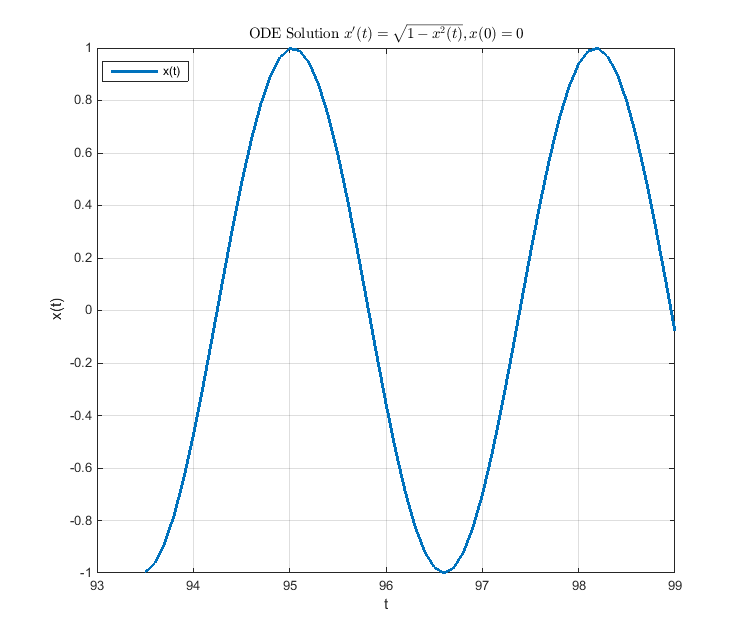
\includegraphics[width=10cm]{ODE1}}
\end{center}
\end{frame}
}
\addtocounter{framenumber}{-1}
{
\begin{frame}[c]{Stochastic approximation algorithms: Example}
\begin{center}
{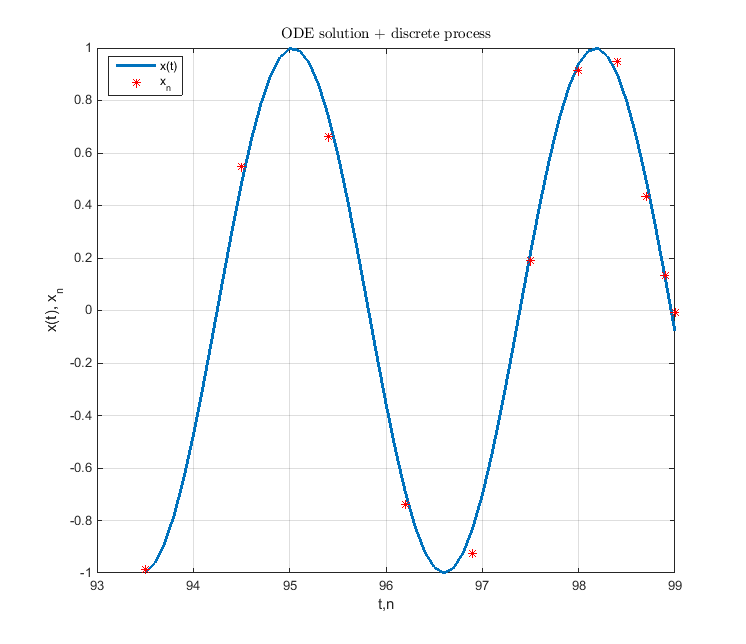
\includegraphics[width=10cm]{ODE2}}
\end{center}
\end{frame}
}
\addtocounter{framenumber}{-1}
{
\begin{frame}[c]{Stochastic approximation algorithms: Example}
\begin{center}
{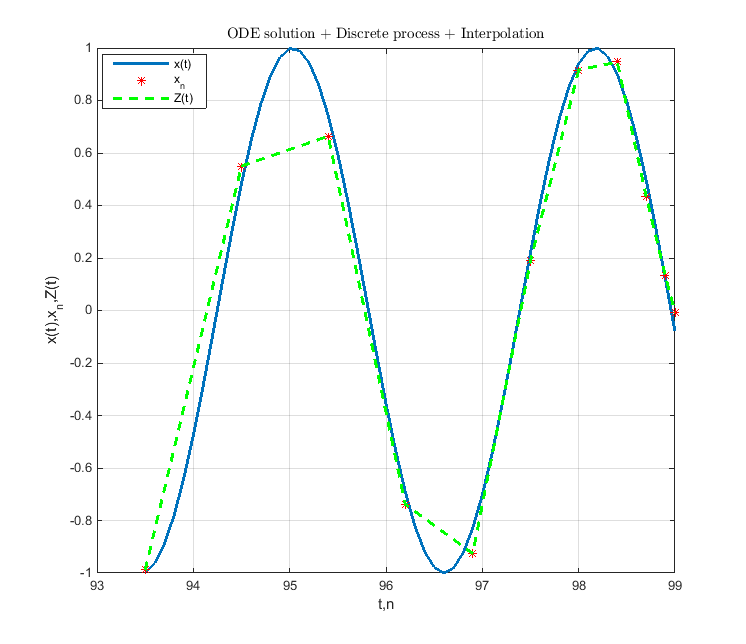
\includegraphics[width=10cm]{ODE3}}
\end{center}
\end{frame}
}

%%%%%%%%SEPARATOR%%%%%%%%% RESULTS 
\addtocounter{framenumber}{-1}
{	
\setbeamertemplate{sidebar right}{\llap{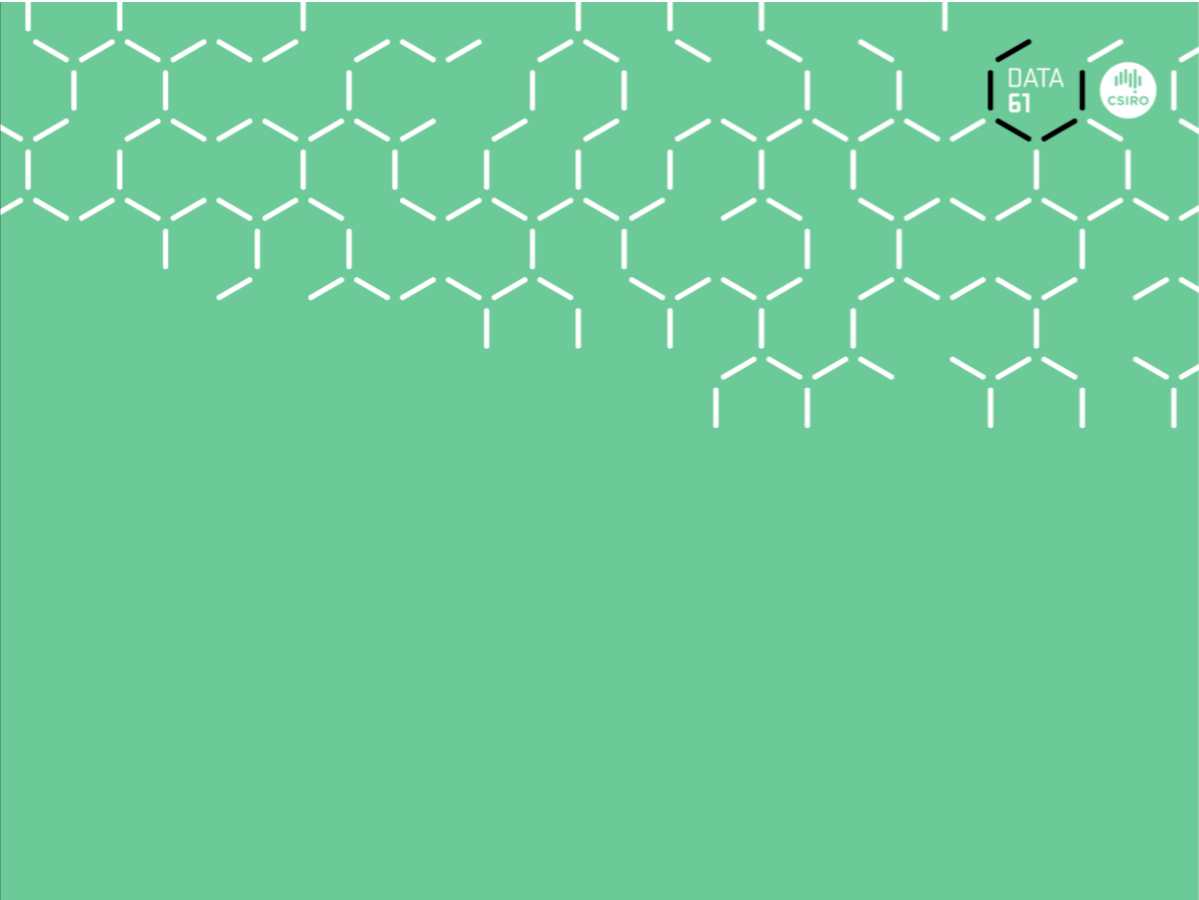
\includegraphics[width=\paperwidth,height=\paperheight]{separator}}}
\begin{frame}[c]
\begin{center}

	\vspace{10em}
	 
\includegraphics[height=0.7cm]{Results}\\
	\vspace{.5em}
	
\end{center}
\end{frame}
}


%%%%%%%%%% MARKET SHARE AS RMA %%%%%

\begin{frame}[c]{Market share as a Robbins Monro Algorithm}
If  $D^k = \sum_{t=0}^k \sum_{i=1}^n d_i^t$
\[\phi^{k} = \frac{D^k \phi^k}{D^k } \Rightarrow
\phi^{k+1} = \frac{D^k \phi^k}{D^k + 1} + \frac{e^k}{D^k + 1}
\]
It follows that 
\begin{align*}
\phi^{k+1} & =  \frac{(D^k+1) \phi^k}{D^k + 1} - \frac{\phi^k}{D^k + 1}  + \frac{e^k}{D^k + 1} \\
       %   & =  \phi^k + \frac{1}{D^k + 1} (e^k - \phi^k) \\
          & =  \phi^k + \frac{1}{D^k + 1} (\EE[e^k | \phi^k] - \phi^k + e^k - \EE[e^k | \phi^k]) \\
          & =  \phi^k + \underbrace{\frac{1}{D^k + 1}}_{\gamma^{k+1} } (\underbrace{p(\phi^k) - \phi^k}_{F(\phi^k) } + \underbrace{e^k - \EE[e^k | \phi^k]}_{U^{k+1}}).
\end{align*}
Continuous dynamic given by
\begin{equation}
\label{RMC-MS}
\frac{d\phi^t}{dt}= p(\phi^t) - \phi^t \quad (\phi^t \in \Delta^{n-1}) 
\end{equation}

\end{frame}


%%%%%%%%%%dynamic equilibria %%%%%

\begin{frame}[c]{Equilibria}
\begin{exampleblock}{Theorem 2.} 
\label{eqs}
Let $f(x)=x^r, 0<r<1$. Then, there is a unique equilibrium to Equation \eqref{RMC-MS} 
in $int(\Delta^{n-1})$, the interior of the simplex, specified by 
\[
\phi^*=\dfrac{1}{\sum_j
  \overline{q}_j^{\frac{1}{1-r}}}[\overline{q}_1^{\frac{1}{1-r}},...,\overline{q}_n^{\frac{1}{1-r}}]
\]
The remaining equilibria are on the boundary of the simplex.
\end{exampleblock}


\textcolor{anugold}{\textit{Remark:}}
If assume that there exists a set $Q\subset \{1,..,n\}$
($|Q|<n$) of indexes such that $\phi_i=0$ if $i\in Q$. The remaining coordinates are given as follows: If $j \notin
Q$, then we have
\[
\phi_j=\frac{\overline{q}_j^{1/(1-r)}}{\sum_{i\notin Q}\overline{q}_i^{1/(1-r)}}.
\]

%
%\begin{exampleblock}{Lemma 2.}
%\label{induction}
%Consider a trial-offer market defined by $n$ items and the submarket
%obtained by considering only $n-1$ items.  This submarket can also be
%modeled by an RMA. 
%\end{exampleblock}
\end{frame}


%%%%%%%%%%CONVERGENCE r<1, UNSTABILITY r>1%%%%%

\begin{frame}[c]{Equilibria and stability}
\begin{exampleblock}{Main Theorem} 
\label{thm:ict} 
Under the social signal $f(x)=x^r, 0<r<1$ with $\phi^0\in
int(\Delta^n)$, the RMA $\{\phi^t\}_{t>0}$ converges to $\phi^*$
almost surely.
\end{exampleblock}

\begin{center}
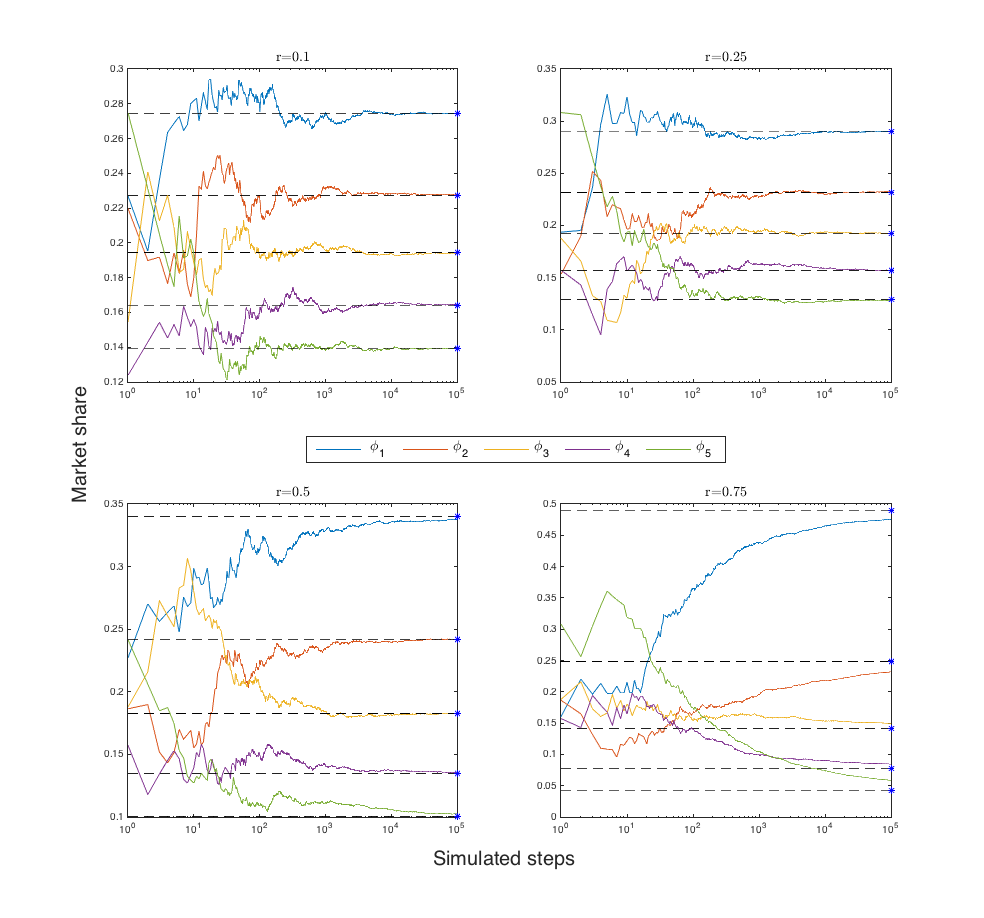
\includegraphics[scale=0.2]{Convergence10x5ItIND}
\end{center}



\end{frame}

%%%%%%%%%%CONVERGENCE r>1%%%%%

\begin{frame}[c]{Equilibria}
\begin{block}{Proposition: (Renlund2010)}
Consider a one-dimentional RMA with $F(x)=p(x)-x$. A point $x^*$ is unstable if there exists a neighbourhood $N_{x^*}$ around $x^*$ such that $F(x)[x-x^*]\geq 0$ for all $x\in N_{x^*}$.
\end{block}

\begin{exampleblock}{Theorem 4.}
\label{unstable}
For a social signal $f(x)=x^r$ with $r>1$, the inner equilibrium is unstable.
\end{exampleblock}


\begin{exampleblock}{Theorem 5.}

Consider the social signal $f(x)=x^r$ with $r>1$. The RMA $\{\phi^t\}_{t \geq 0}$ converges almost surely to one of the equilibria $\phi\in Z_F:=\{x\in \Delta^{n-1}: p(x)-x=0\}$.
\end{exampleblock}
\end{frame}




%%%%%%%%%%PLOTS PREDICT%%%%%

\begin{frame}[c]{Predictability plots}
\begin{center}
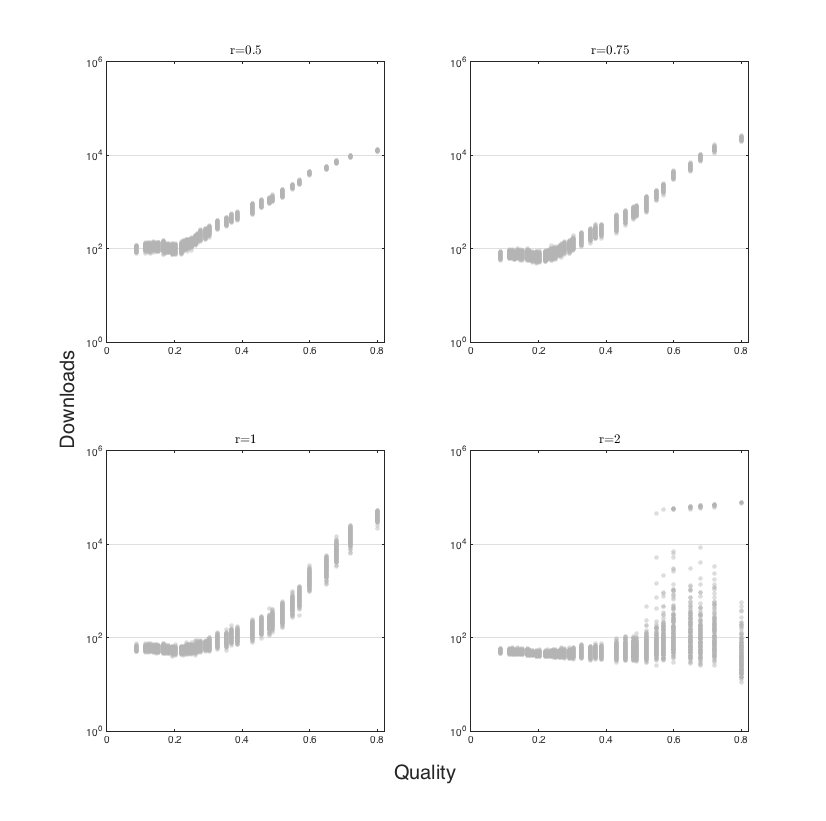
\includegraphics[scale=0.3]{predict200expeNegCorrQrank10x5it}
\end{center}


\end{frame}


%%%%%%%%SEPARATOR%%%%%%%%% PROGRESS
\addtocounter{framenumber}{-1}
{	
\setbeamertemplate{sidebar right}{\llap{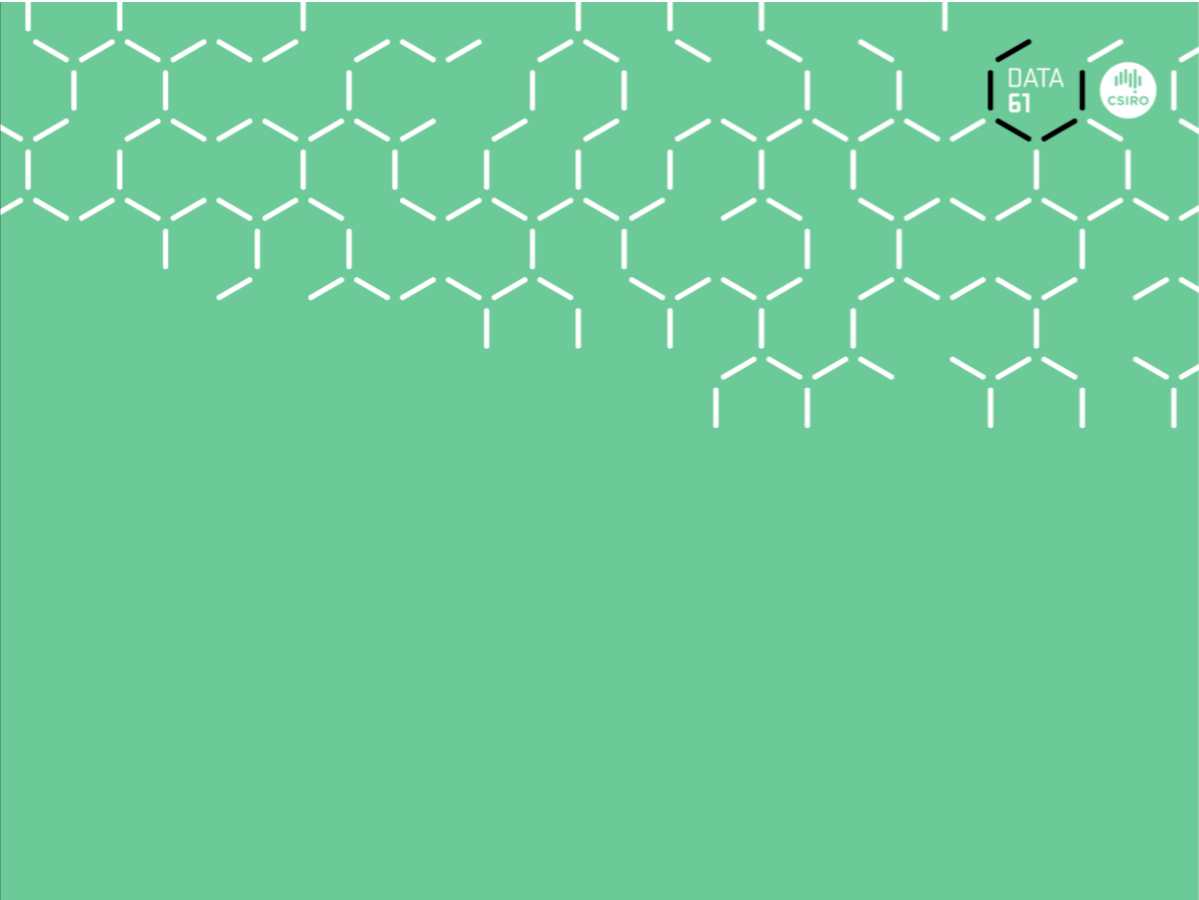
\includegraphics[width=\paperwidth,height=\paperheight]{separator}}}
\begin{frame}[c]
\begin{center}

	\vspace{10em}
	 
\includegraphics[height=1.5cm]{Progress}\\
	\vspace{.5em}
	
\end{center}
\end{frame}
}



%%%%%%%%%% ARTICLE JOURNAL OR, CONFERENCE PAPER I%%%%%

\begin{frame}[c]{Submitted and accepted papers}

\begin{block}{Submitted}
\begin{itemize}
\item Popularity Signals in Trial-Offer Markets. Operations Research.
\item Asymptotic Optimality of Myopic Optimization in Trial-Offer Markets with Social Influence. 25th International Joint Conference on Artificial Intelligence (IJCAI16 New York City, USA. July 9-15). 
\end{itemize}
\end{block}

\begin{block}{Accepted}
 Aligning Popularity and Quality in Online Cultural Markets.The 10th International Conference of Web and Social Media (ICWSM 2016- Cologne, Germany. May 17-20).
\end{block}

\begin{block}
{Second Workshop on Algorithms and Dynamics for Games and Optimization. Santiago, Chile. Jan 25-29.}
\end{block}



\end{frame}



%%%%%%%%%% FUTURE WORKI%%%%%

\begin{frame}[c]{Current and future work}
\begin{itemize}
\item Asymptotic study of popularity rankings (in progress, I will continue it during my visit to University of Michigan).
\item {\it Side project:} Develop a formal generalisation of Polya Urn (currently well studied only for the case of 2 colors).
\item Using the convergence results for sublinear functions using static rankings, create an alternative way to recover qualities*.
\end{itemize}

\begin{alertblock}{Scheme:}
\begin{enumerate}
\item Define a time horizon (e.g 1 week), and divide it in 9 steps.
\item Order the songs according to some previous information (or random) and apply a social signal $f(x)=x^{0.1}$.  Using the convergence theorem compute the values of $q_{i,1}$.
\item Order the songs using the values of $q_{i,1}$ and apply a social signal $f(x)=x^{0.2}$, obtaining $q_{i,2}$.
\item Repeat for the remaining values of $r \in \{0.3,...., 0.9\}$.
\end{enumerate}
\end{alertblock}


\end{frame}


{	
\setbeamertemplate{sidebar right}{\llap{
\includegraphics[width=\paperwidth,height=\paperheight]{Opening}}}
\begin{frame}[c]
\begin{center}

	\vspace{10em}
	 
\includegraphics[height=1cm]{Thanks}\\
	\vspace{.5em}
	
\end{center}
\end{frame}
}


%%%BACKUP SLIDES 1

\addtocounter{framenumber}{-1}
{
\begin{frame}[c]
{\it Proof of Theorem 2}
We know the equilibria are given by $p(x)=x\Leftrightarrow p_i(x)=x_i, \forall i\in\{1,...,K\} $, then
	
%%%% equilibria	
	$p_i(\Phi)=\phi_i\Leftrightarrow \frac{\overline{q}_i(\phi_i)^r}{\sum_{j=0}^K\overline{q}_j(\phi_j)^r}=\phi_i$\\
	if  $\phi_i>0$ for all $i$, and then we have the following:
	$p_i(\Phi)=\phi_i\Leftrightarrow \overline{q}_i(\phi_i)^{r-1}=\sum_{j=0}^K\overline{q}_j(\phi_j)^r,$\\
	then 	\begin{equation*}
	\overline{q}_i(\phi_i)^{r-1}=\overline{q}_j(\phi_j)^{r-1}\Leftrightarrow \phi_i=\left(\frac{\overline{q}_i}{\overline{q}_j}\right)^{\frac{1}{1-r}}\phi_j
	\end{equation*}
	
	Adding from $i=1$ to $i=K$ we have
	$1=\sum_{i=1}^K\phi_i=\frac{\phi_j}{\overline{q}_j^{1/(1-r)}}\sum_{i=1}^K\overline{q}_i^{1/(1-r)},$
	and in consecuence
	$\phi_j=\frac{\overline{q}_j^{1/(1-r)}}{\sum_{i=1}^K\overline{q}_i^{1/(1-r)}},\quad j\in \{1,...,K\} $ are the coordinates of the equilibrium.

\end{frame}



%%%BACKUP SLIDES 2

\addtocounter{framenumber}{-1}
{
\begin{frame}[c]
{\it Proof of Theorem 3}
The proof studies the asymptotic behaviour of the solutions of the following ODE:
\begin{equation}
\label{ODEE}
\frac{d \phi^t}{dt}=p(\phi^t)-\phi^t.
\end{equation}

Hence, we have
\begin{align*}
&\frac{\overline{q}_i(\phi_i^t)^r}{\sum_j\overline{q}_j(\phi_j^t)^r}=\frac{d\phi_i^t}{d t}+\phi_i^t, \\
&\frac{1}{\sum_j\overline{q}_j(\phi_j^t)^r}=\frac{1}{\overline{q}_i(\phi_i^t)^r}[\frac{d\phi_i^t}{d t}+\phi_i^t] \quad \mbox{ if } \phi_i^t\neq 0,\\
&\overline{q}_i^{-1}[(\phi_i^t)^{-r}\frac{d\phi_i^t}{d t}+(\phi_i^t)^{1-r}]=\overline{q}_j^{-1}[(\phi_j^t)^{-r}\frac{d\phi_j^t}{d t}+(\phi_j^t)^{1-r}], \\
&\frac{d}{dt}\left[ e^{(1-r)t}\overline{q}_i^{-1}(\phi_i^t)^{1-r}\right]=\frac{d}{dt}\left[ e^{(1-r)t}\overline{q}_j^{-1}(\phi_j^t)^{1-r}\right]
\end{align*} 



\end{frame}
}



%%%BACKUP SLIDES 3

}\addtocounter{framenumber}{-1}
{
\begin{frame}[c]
Integrating and re-ordering  terms we have:
\begin{equation}
\label{equili}
\frac{(\phi_i^t)^{1-r}}{\overline{q}_i}-\frac{(\phi_j^t)^{1-r}}{\overline{q}_j}= e^{(r-1)t}\left[   \frac{(\phi_i^0)^{1-r}}{\overline{q}_i}-\frac{(\phi_j^0)^{1-r}}{\overline{q}_j} \right].
\end{equation}

if $\displaystyle
  \frac{(\phi_i^0)^{1-r}}{\overline{q}_i}\neq\frac{(\phi_j^0)^{1-r}}{\overline{q}_j}$,
  the right-hand side of Equation \eqref{equili} goes to zero as $t\to \infty$  (because
  $r<1$) and hence
\begin{equation}
\label{limit}
\lim_{t\to\infty} \frac{(\phi_i^t)^{1-r}}{\overline{q}_i}-\frac{(\phi_j^t)^{1-r}}{\overline{q}_j}=0. 
\end{equation}

Now denote by $\phi_j$ the limit of $\phi_j^t$ for all $j \in
\{1,...,n\}$. Using Equation \eqref{limit}, the following equation holds for all $i,j
\in\{1,...,n\}$:
\begin{equation}
\frac{\phi_{i}^{1-r}}{\overline{q}_i}=\frac{\phi_{j}^{1-r}}{\overline{q}_j} \Leftrightarrow \phi_{i}=\frac{\phi_{j}}{\overline{q}_j^{1/(1-r)}}\overline{q}_i^{1/(1-r)}
\end{equation}

which is the equation that defines $\phi^*$ in Theorem 2.

\end{frame}
}

